%-------------------------------------------------------------------
\chapter{Interactive platform with Streamlit}
\label{c:streamlit}
%-------------------------------------------------------------------

To make the results of the Mixture NCA experiments easy to explore and to support a direct visual comparison between model predictions and ground truth, an interactive web application was built using Streamlit.
This chapter outlines the motivations for this choice, what the platform is and what it is used for, how it was developed, its main functionalities (with screenshots), and why the predictions shown in the interface do not align fully with the true ground truth.
It also explains why the dashboard is set up to display only the results of the latest curriculum learning experiment.

%----------------------------------------------------------
\section{Motivations and role of Streamlit}
%----------------------------------------------------------

Streamlit is an open-source framework for building web interfaces for data science and machine learning applications from Python scripts, without writing HTML, CSS or JavaScript.
Its adoption in this work was driven by practical needs.
First, the experiments described in Chapter~\ref{c:implementation} produce a large amount of data: trained checkpoints for different neighborhood sizes, aggregated biological metrics, and simulation trajectories that are naturally explored in an interactive way.
Making these results available through a self-contained application allows users to pick an experiment, load a checkpoint, run a rollout and compare the model output with the simulator trajectory frame by frame, without re-running command-line scripts or opening notebooks each time.
Second, Streamlit makes it possible to obtain a usable interface quickly: widgets such as sliders, select boxes, tabs and expanders, as well as column layouts, are built in, and integration with libraries like Plotly for charts and PyTorch for loading models is straightforward.
Finally, the application can be run locally and, if desired, deployed on platforms such as Streamlit Cloud or an internal server, keeping a single codebase for both analysis and demonstration.

In our setting, the platform serves a dual purpose: it is a tool for \emph{testing and inspecting} trained models (choosing the experiment, model type and initial state, and viewing the rollout alongside ground truth), and at the same time a \emph{dashboard} that aggregates metrics and experiment configuration by neighborhood size and model type, in line with the folder structure produced by the curriculum learning pipeline described in Chapter~\ref{c:implementation}.

%----------------------------------------------------------
\section{Development and architecture}
%----------------------------------------------------------

The application is organised around a small set of components: a main entry point that handles page configuration and navigation, a layer responsible for loading trained models and running rollouts, and a dashboard layer that discovers and aggregates experiment outputs.

The main component sets the page layout (wide, with an expanded sidebar), keeps session state for rollout frames and for a cache of loaded models, and provides navigation between two views via a sidebar radio control: ``Model test'' and ``Experiments dashboard''.
By default, the application reads from the results directory produced by the curriculum learning pipeline.
Inside that directory it looks for subfolders named by neighborhood size (e.g.\ \texttt{NB\_2}, \texttt{NB\_3}, \texttt{NB\_5}) and uses them as the list of available experiments.

Model loading and rollout execution are handled by a dedicated module.
For each experiment folder, the application looks for final checkpoints (excluding intermediate phase checkpoints), infers the neighborhood size from the folder name, and instantiates the corresponding Mixture NCA or Stochastic Mixture NCA with the same architecture as in training.
The rollout is run from an initial state given as a grid of cell types (e.g.\ taken from the same history dataset used in training), with a configurable number of steps (up to 500) and, for the stochastic model, an optional seed for reproducibility.
The resulting frames are converted to RGBA images for display (mapping cell types to the colours defined in the tissue model) and shown side by side with ground-truth frames when the latter are available.

The dashboard component scans the results directory, reads for each neighborhood-sized subfolder the stored configuration and curriculum metadata and the computed biological metrics (per step length and model type), and builds a structured representation of each experiment.
Metrics from all experiments can be aggregated into a single table or visualised with interactive charts (e.g.\ KL divergence, Chi-Square, Categorical MMD, tumor size difference, border size difference, spatial variance difference).

%----------------------------------------------------------
\section{Functionality and screens}
%----------------------------------------------------------

\paragraph{Model test.}
On the ``Model test'' page the user selects in the sidebar the results folder, the experiment (neighborhood size), the model type (Mixture NCA or Stochastic Mixture NCA), and optionally the history dataset and the simulation and initial-frame indices.
A ``Simulate'' button starts the rollout; when it finishes, a confirmation message appears (e.g.\ ``Simulation completed: 500 frames'') and a ``Frame'' slider allows stepping through time.
For each selected step, two images are shown side by side: on the left the ground-truth frame from the simulator, on the right the frame predicted by the model at that step.
Grids are rendered with nearest-neighbour interpolation (pixelated) so that discrete cells remain visually clear.

Figure~\ref{fig:streamlit:model_test_step0} shows the interface at the initial step (step 0): the initial state is the same for both columns (same seed or history), but even at this frame small differences can appear due to how the model represents and evolves the state.
Figures~\ref{fig:streamlit:model_test_step177} and~\ref{fig:streamlit:model_test_step499} show the same comparison at steps 177 and 499.
As time advances, the shape and distribution of cell types (in particular the red cells, typically differentiated or in transition) in the prediction can diverge from the real trajectory: the predicted structure often looks more fragmented, with red pixels more spread inside the tissue, whereas in the ground truth red cells tend to concentrate along the boundaries and in more defined regions.
This kind of mismatch is exactly what is discussed in Section~\ref{sec:streamlit:alignment} and has already been analysed from a methodological standpoint in \cref{sec:impl:curriculum:limitations}.

\begin{figure}[H]
  \centering
  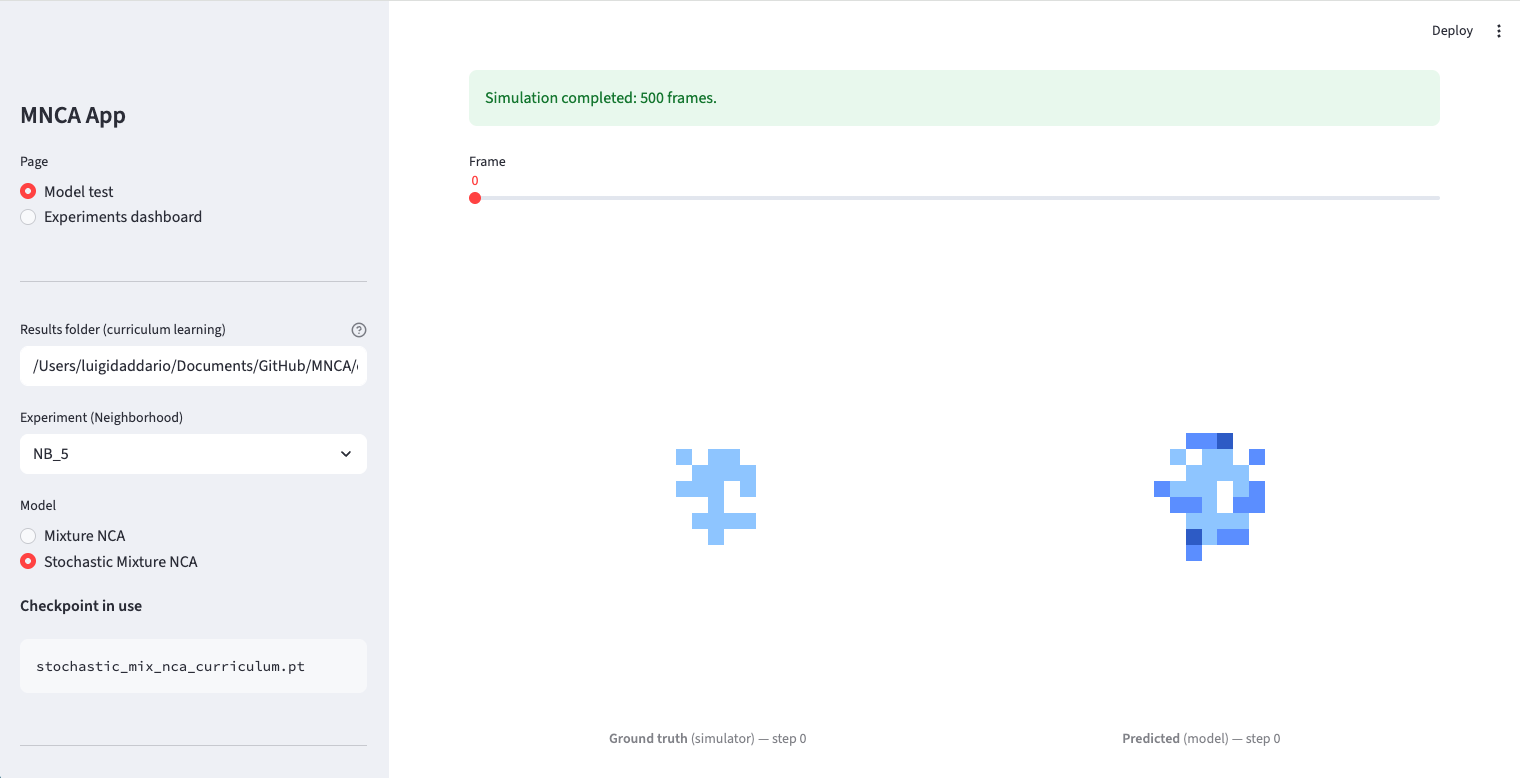
\includegraphics[width=0.95\textwidth]{figs/streamlit/streamlit_model_test_step0.png}
  \caption{``Model test'' page of the MNCA platform: comparison of ground truth (left) and prediction (right) at step 0. Sidebar: experiment (e.g.\ neighborhood 5), model (Stochastic Mixture NCA) and checkpoint in use.}
  \label{fig:streamlit:model_test_step0}
\end{figure}

\begin{figure}[H]
  \centering
  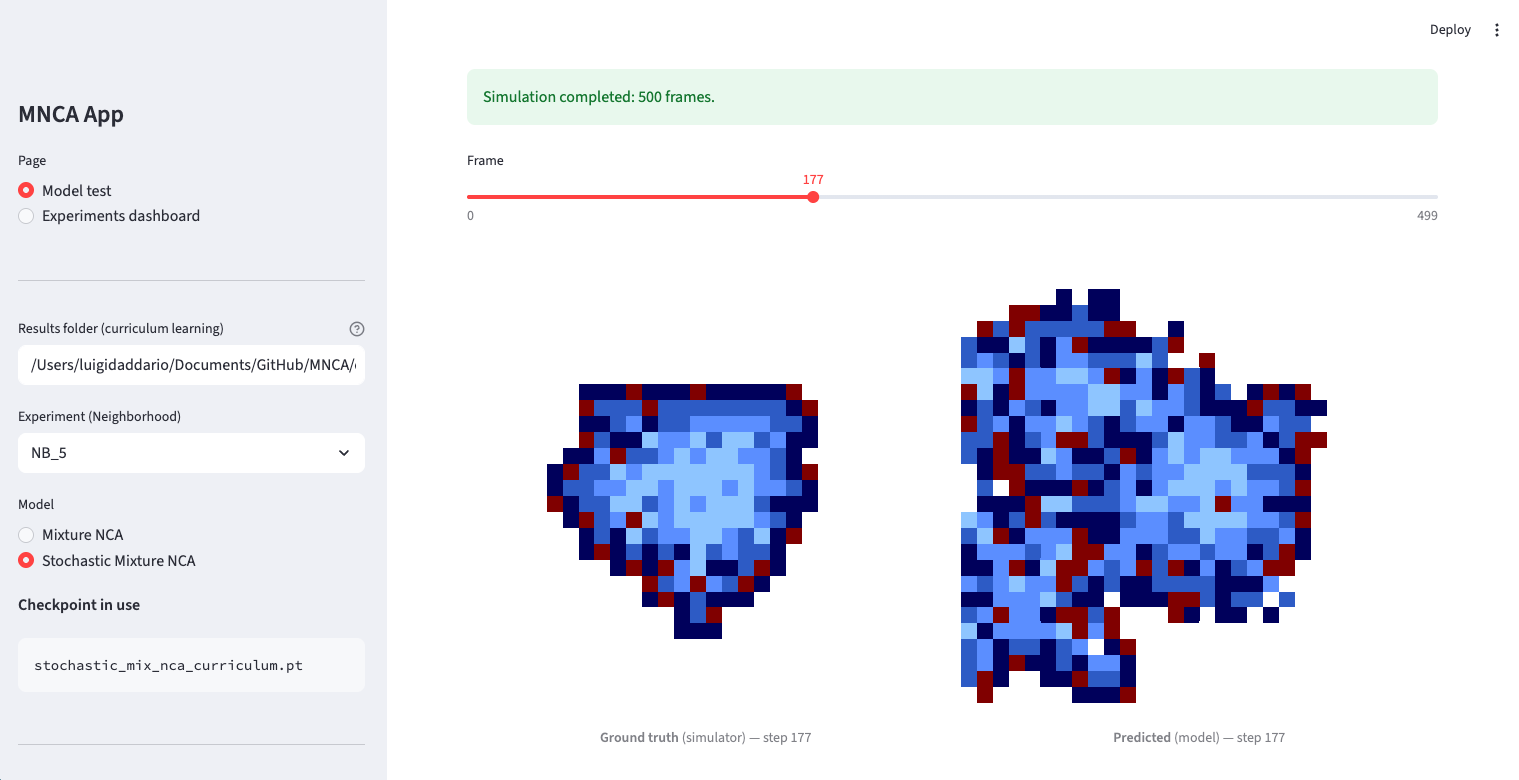
\includegraphics[width=0.95\textwidth]{figs/streamlit/streamlit_model_test_step177.png}
  \caption{Same Model test session at step 177. The prediction (right) begins to show a slightly different cell-type distribution and morphology compared to the ground truth (left).}
  \label{fig:streamlit:model_test_step177}
\end{figure}

\begin{figure}[H]
  \centering
  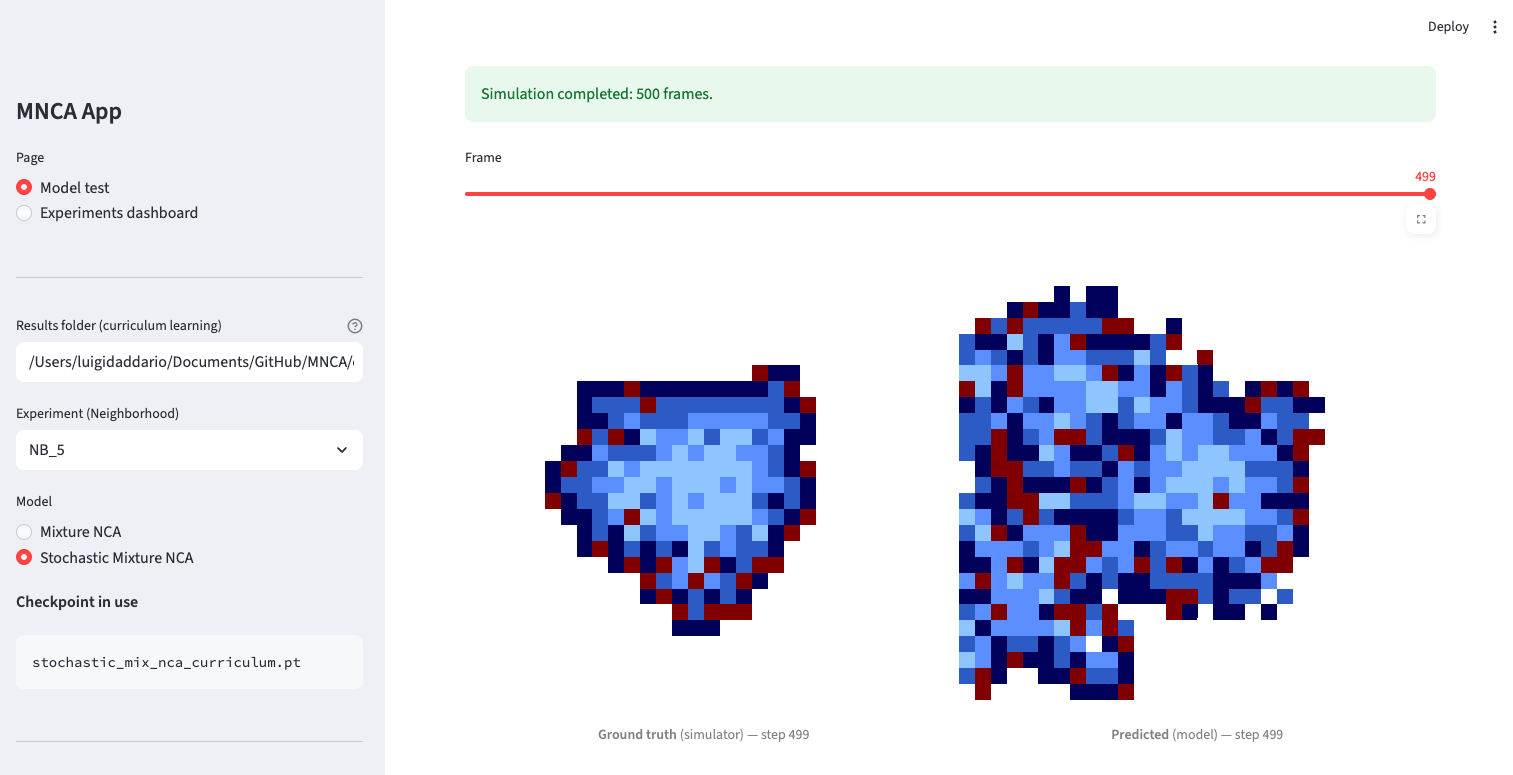
\includegraphics[width=0.95\textwidth]{figs/streamlit/streamlit_model_test_step499.png}
  \caption{Comparison at step 499 (end of rollout). The divergence between prediction and ground truth is more pronounced: less compact structure and greater spread of red pixels in the prediction.}
  \label{fig:streamlit:model_test_step499}
\end{figure}

\paragraph{Experiments dashboard.}
The ``Experiments dashboard'' page provides an aggregated view by neighborhood size and model type.
In the sidebar the user can set the results directory; the application reports how many experiment subfolders it found.
The main area has three tabs: an experiment summary (per neighborhood), a full metrics table, and overview charts.

In the summary tab, each experiment is shown in an expandable block with the neighborhood identifier and size.
Inside are the configuration (training parameters, curriculum), the list of saved checkpoints (final results only, no phase checkpoints), and the biological metrics both as a table and as charts (metrics vs.\ step length for that neighborhood).
Figure~\ref{fig:streamlit:dashboard_summary} shows an example with one neighborhood expanded and the curriculum section visible (time length, epochs, learning rate per phase).

In the metrics tab, all metrics from the discovered experiments are merged into a single table (Figure~\ref{fig:streamlit:dashboard_metrics}), with columns for model type, KL Divergence, Chi-Square, Categorical MMD, Tumor Size Diff, and so on, with standard deviations when available.
This allows a quick comparison across neighborhood sizes and between Mixture NCA and Stochastic Mixture NCA.
The overview charts tab displays the same data graphically (via Plotly), with one subplot per metric.

\begin{figure}[H]
  \centering
  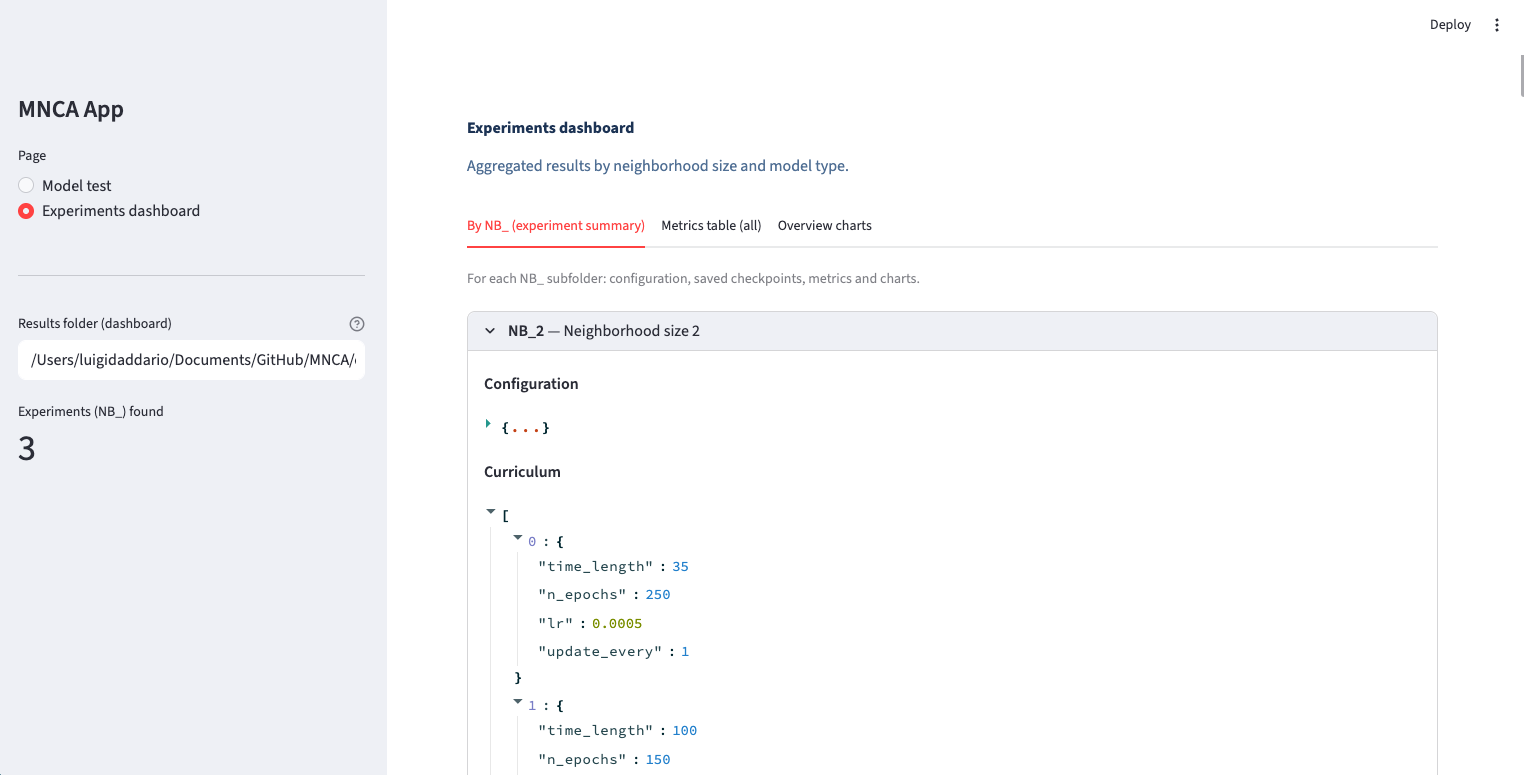
\includegraphics[width=0.95\textwidth]{figs/streamlit/streamlit_dashboard_summary.png}
  \caption{Experiments dashboard, summary tab: detail for one neighborhood with configuration and curriculum (time length, epochs, learning rate per phase).}
  \label{fig:streamlit:dashboard_summary}
\end{figure}

\begin{figure}[H]
  \centering
  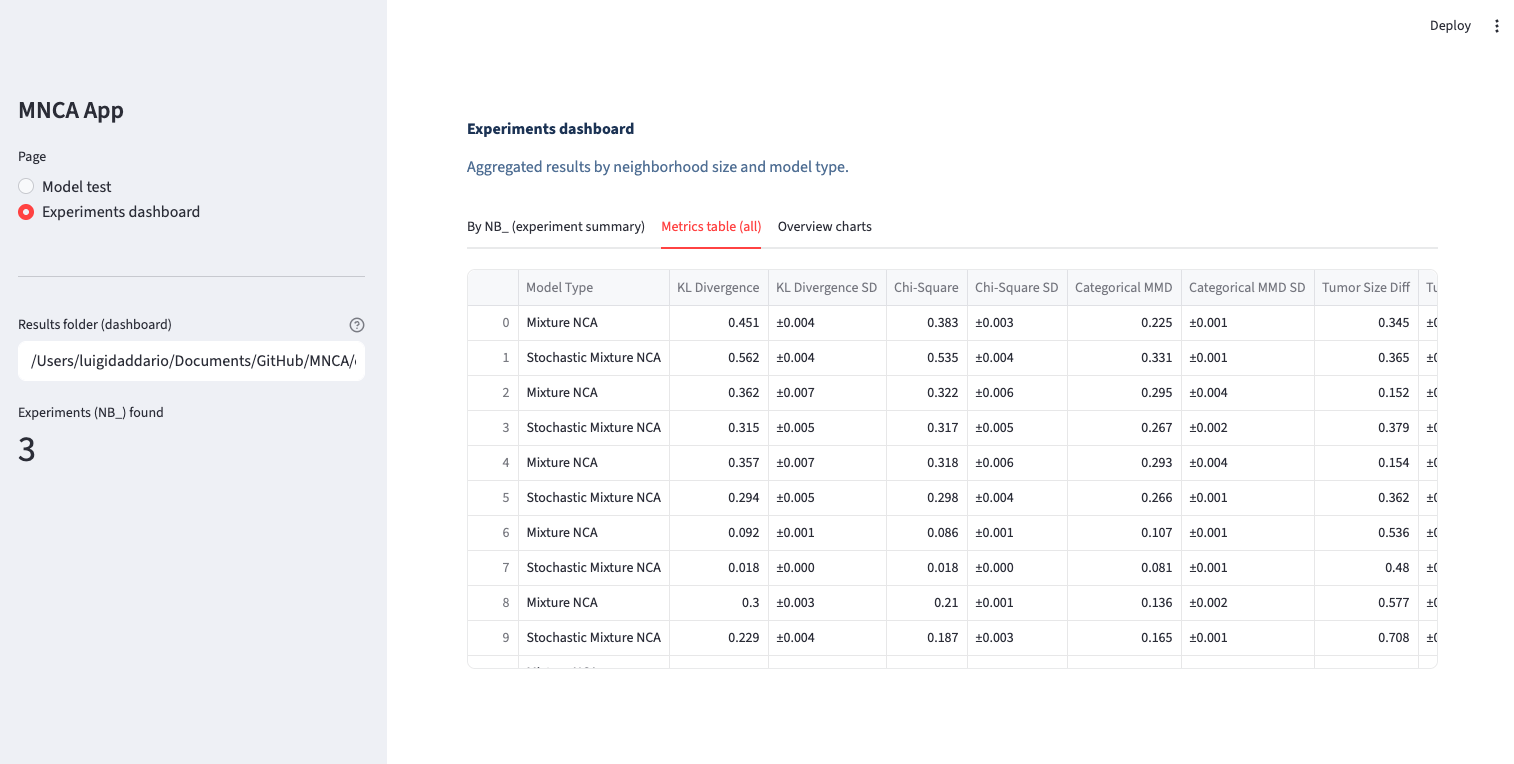
\includegraphics[width=0.95\textwidth]{figs/streamlit/streamlit_dashboard_metrics.png}
  \caption{Experiments dashboard, metrics tab: aggregated table of metrics (KL Divergence, Chi-Square, Categorical MMD, Tumor Size Diff, etc.) for all experiments and model types.}
  \label{fig:streamlit:dashboard_metrics}
\end{figure}

%----------------------------------------------------------
\section{Why the prediction does not align with ground truth}
\label{sec:streamlit:alignment}
%----------------------------------------------------------

When viewing the frame-by-frame comparison on the Model test page, it is clear that the trajectory generated by the model does not match the simulator trajectory, especially at later steps.
This misalignment is not a flaw of the interface but reflects inherent limitations in how the models are trained and evaluated, already discussed in \cref{sec:impl:curriculum:limitations}; here we give a concise, user-oriented reading of the same phenomena.

During training, teacher forcing is used: at each step the model receives the \emph{true} state from the training history, so errors do not accumulate and the loss can stay low.
At test time, by contrast, free rollouts are run: the model receives only its own previous output as input.
A small error at step 10 is then fed into step 11 and so on; after hundreds of steps the trajectory can drift noticeably from the ground truth even if the model has learned the local dynamics well.
In other words, the loss that is optimised is a step-by-step mean squared error over the training window; it encourages correct prediction of the next state given the current one, but does not directly reward the fact that an entire free trajectory matches a single simulator realisation.
It is therefore possible to have a model with low loss and at the same time clear drift when it is run autonomously.

For the Stochastic Mixture NCA there is an additional factor: at each step a rule is sampled, so different runs with different seeds produce different trajectories.
The ground truth we compare against is only one possible realisation of the stochastic simulator; part of the ``difference'' we see is thus natural variability between realisations, not only model error.
Even so, the figures often show an over-abundance of differentiated (red) cells and a less compact structure in the prediction, indicating that the model has not yet perfectly learned the long-horizon dynamics.

Finally, the last phase of the curriculum uses 500-step windows but with fewer epochs and a reduced learning rate; training may stop before the model has fully stabilised behaviour over the full horizon, contributing to the gap observed at the final steps.
The Streamlit platform makes this phenomenon directly visible and interpretable without re-running evaluation scripts.

%----------------------------------------------------------
\section{Choice of results shown in the dashboard}
%----------------------------------------------------------

The application is configured to read results from a single root directory, the one produced by the curriculum learning pipeline.
Within it, all subfolders corresponding to neighborhood sizes are detected; the dashboard then aggregates whatever is present in that directory (configuration, checkpoints, metrics).

In this thesis we have chosen to use the platform with the results of the \emph{latest} curriculum experiment, i.e.\ the one whose parameters and metrics are described in Chapter~\ref{c:implementation} and discussed in the results.
In this way the dashboard does not mix runs from different campaigns (e.g.\ earlier neighborhood sweeps or experiments with different history lengths), but reflects a single coherent set of runs: the same training conditions, the same history dataset and the same curriculum phases.
A user opening the application therefore sees exactly the results that underpin the experimental part of the thesis, and can inspect for each neighborhood the configuration, saved checkpoints and biological metrics, and test the models interactively by loading initial states from the same histories used in training.
If in the future other experiments were to be included, it would suffice to point the results folder to another path or to combine several directories into one; the application logic would remain the same and would continue to discover all neighborhood-sized subfolders in the configured directory.
